% This file was created with tikzplotlib v0.10.1.
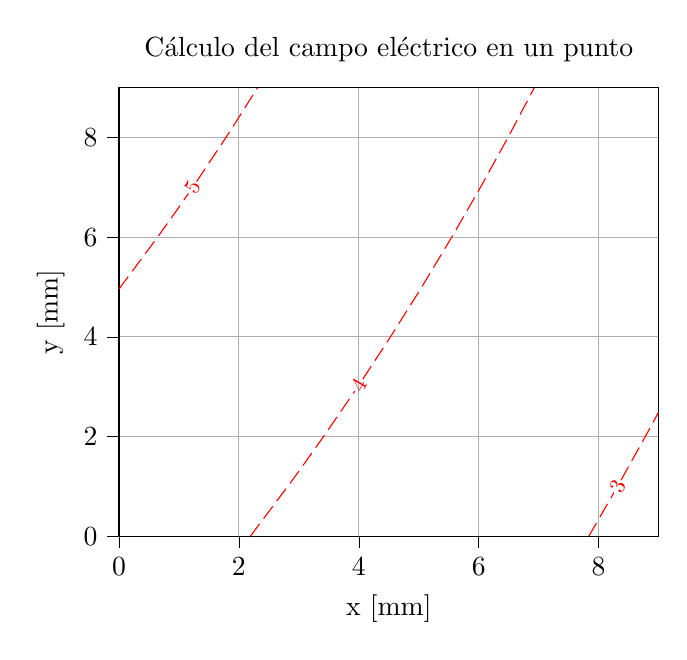
\begin{tikzpicture}

\definecolor{darkgray176}{RGB}{176,176,176}

\begin{axis}[
tick align=outside,
tick pos=left,
title={Cálculo del campo eléctrico en un punto},
x grid style={darkgray176},
xlabel={x [mm]},
xmajorgrids,
xmin=0, xmax=9,
xtick style={color=black},
y grid style={darkgray176},
ylabel={y [mm]},
ymajorgrids,
ymin=0, ymax=9,
ytick style={color=black}
]
\addplot [dash pattern=on 5.55pt off 2.4pt, draw=none, draw=red]
table{%
x  y
7.83480035577106 0
8 0.338837660336923
8.25506123520785 0.875237333912917
};
\addplot [dash pattern=on 5.55pt off 2.4pt, draw=none, draw=red]
table{%
x  y
8.37247058148563 1.12537664522648
8.77766235214623 2
9 2.49140114639821
};
\addplot [dash pattern=on 5.55pt off 2.4pt, draw=none, draw=red]
table{%
x  y
2.19051588081864 0
2.81518337474896 1
3 1.30360051004054
3.41154509336013 2
3.93195813804583 2.91250051862379
};
\addplot [dash pattern=on 5.55pt off 2.4pt, draw=none, draw=red]
table{%
x  y
4.06598599747269 3.15366916366391
4.52681121491503 4
5 4.90511978901095
5.04849487213474 5
5.54806839191334 6
6 6.9436031263497
6.0265151580163 7
6.48574422069881 8
6.92587373870444 9
};
\addplot [dash pattern=on 5.55pt off 2.4pt, draw=none, draw=red]
table{%
x  y
0 4.96325697714091
0.023360785835511 5
0.641995861432829 6
1 6.60588562796323
1.15843476332525 6.88054036733707
};
\addplot [dash pattern=on 5.55pt off 2.4pt, draw=none, draw=red]
table{%
x  y
1.29425016350205 7.12065479399302
1.78186129828817 8
2 8.41039139028885
2.30779353393258 9
};
\draw (axis cs:8.31438662500134,1) node[
  scale=0.8,
  text=red,
  rotate=64.3
]{3};
\draw (axis cs:4,3.03248225306582) node[
  scale=0.8,
  text=red,
  rotate=60.4
]{4};
\draw (axis cs:1.22734512937617,7) node[
  scale=0.8,
  text=red,
  rotate=59.9
]{5};
\end{axis}

\end{tikzpicture}
